\section{Analyse de l'existant}

PresTaf est un programme codé par M. Jean-Michel Couvreur, qui prend des formules de Presburger en entrées et les résout à l'aide d'automates minimaux. Tout d'abord il génère des automates déterministes et finis mais non minimaux. Il faut donc les minimiser, et pour se faire PresTaf utilise un algorithme d'Hopcroft modifié. L'ensemble des transitions menant de l'état initial vers un état final est solution de la formule. En outre si l'état final est l'état \emph{zero} alors il n'y aucune solution et si l'état final est l'état \emph{one} alors la formule est une tautologie.\\\par

Mona, est une bibliothèque C qui résout des formules monadique. La où PresTaf n'implémente à ce jour que la logique arithmétique de Presburger, la logique monadique pourrait être implémentée dans le futur.\\\par

Lash\cite{lash} est une bibliothèque C qui résout des formules de Presburger mais à la différence de PresTaf, il fonctionne sur des automates infinis. Cette différence induit une importante baisse de performances. En effet pour les mêmes formules, PresTaf était bien plus rapide à s'executer que Lash\cite{DBLP:conf/wia/Couvreur04}.\\\par

Prenons une formule simple, comme $x = y$. Dans cette formule il y a deux variables qui vont devoir être lu simultanément en partans du bit de poids faible, mais imaginons la bibliothèque Prestaf comme une machine de Turing à une seule bande uni-infini. D'instinct on souhaiterai lire deux par deux les bits mais ce n'est pas ce que fait la bibliothèque, à la place c'est comme si la bande alternait les bits de $x$ avec ceux de $y$.\\\par
Prenons par exemple $x = 100110$ et $y = 101$, pour commencer Prestaf ajoute autant de 0 devant que nécessaire pour que $x$ et $y$ fasse la même taille, donc on a $y'=000101$ pour plus de lisibilité je vais noté les bits correspondant à $x$ comme ceci : $b_x$ et respectivement $b_y$. Ainsi la bande construite sera la suivante :

\begin{figure}[h]
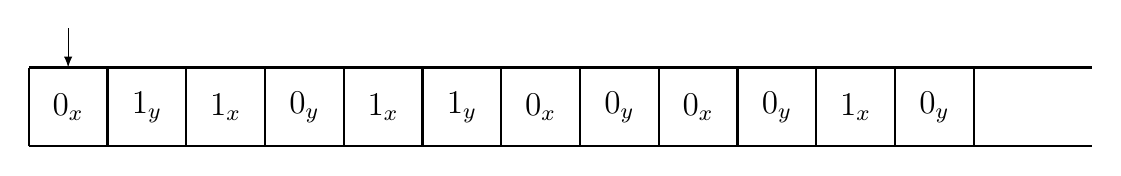
\begin{tikzpicture}
\draw[thick] (0, 0) -- (13.5, 0);
\draw[thick] (0, 1) -- (13.5, 1);
\draw[thick] (0, 0) -- (0, 1);

\foreach \x in {1,...,12} {
	\draw[thick] (\x, 0) -- (\x, 1);
}

\node at (0.5,0.5) {\large $0_x$};
\node at (1.5,0.5) {\large $1_y$};

\node at (2.5,0.5) {\large $1_x$};
\node at (3.5,0.5) {\large $0_y$};

\node at (4.5,0.5) {\large $1_x$};
\node at (5.5,0.5) {\large $1_y$};

\node at (6.5,0.5) {\large $0_x$};
\node at (7.5,0.5) {\large $0_y$};

\node at (8.5,0.5) {\large $0_x$};
\node at (9.5,0.5) {\large $0_y$};

\node at (10.5,0.5) {\large $1_x$};
\node at (11.5,0.5) {\large $0_y$};

\draw[-latex] (0.5, 1.5) -- (0.5, 1);

\end{tikzpicture}

\caption{Bande d'entrée, avec la tête de lecture en $0_x$}
\end{figure}

Comparons maintenant les automates produit par cette formule tels qu'il serait dessiner en lisant deux à deux et en lisant selon cette bande uni-infini. \clearpage

\begin{figure}[h]

\begin{tikzpicture}

\node[circle,draw, accepting] (A) at (0, 0)  {$q_0$};
\node[circle,draw, accepting] (B) at (0, -2)  {$zero$};

\path[->, thick] (0, 1) edge (A)
(A) edge [bend right] node[left]{$0_x1_y$} (B)
(A) edge [bend left] node[right]{$1_x0_y$} (B)
(A) edge [loop left] node[left]{$0_x0_y$} (A)
(A) edge [loop right] node[right]{$1_x1_y$} (A);

\node[circle,draw, accepting] (C) at (8.5, 0)  {$q_0$};
\node[circle,draw] (D) at (7, -2)  {$q_1$};
\node[circle,draw,accepting] (E) at (10, -2)  {$q_2$};
\node[circle,draw, accepting] (F) at (8.5, -4)  {$zero$};

\path[->, thick] (8.5, 1) edge (C)
(C) edge [bend left] node[right]{$0_x$} (E)
(E) edge [bend left] node[right]{$0_y$} (C)
(C) edge [bend left] node[right]{$1_x$} (D)
(D) edge [bend left] node[left]{$1_y$} (C)
(D) edge node[left]{$0_y$} (F)
(E) edge node[right]{$1_y$} (F);

\end{tikzpicture}


\caption{À gauche l'automate "instictif", à droite l'automate produit par PresTaf}
\end{figure}

Le nombre d'état s'en voit bien entendu multiplié, comme on ne lit pas simultanément les bits. Revenons-en à notre bande $x = 100110$ et $y = 101$, ici bien entendu les nombres ne sont pas égaux, si sur l'automate de gauche le résultat est immédiat, pour l'automate de droite il va d'abord se déplacé dessus avant d'arrivé en 0. Cette écriture en "alternance" peut rendre rapidement les automates très grands, et peu lisible, cependant ceci permet un alphabet unique de taille 2.\\\par

En effet avec l'exemple à deux variables, si l'on lisait les bits simultanément on aurait l'alphabet suivant : $\Sigma = \{00, 01, 10, 11\}$, pour une formule à trois variables on aurait $|\Sigma| = 8$, et ainsi de suite, en lisant chaque bits simultanément on aura un alphabet de taille exponentiel en la taille de l'entrée. Si l'on à $n$ variables, on aurai $|\Sigma| = 2^n$. En prenant un tel alphabet, la minimisation d'automate serait beaucoup plus complexe, plus longue et plus couteuse en espace. Qui plus est, en ayant un alphabet unique ceci facilite grandement les prédictions en espace et en mémoire. Tandis qu'un alphabet a taille variables ajoute un paramètre de compléxité qui n'est pas désiré.
